\documentclass{git_course}

\begin{document}

\author{Paul Cochrane}
\title[Version control with Git]
        {Version control with Git}
\date{\today}

\maketitle

\begin{frame}
\begin{multicols}{2}
\begin{spacing}{0.8}
\tableofcontents
\end{spacing}
\end{multicols}
\end{frame}


%%%%%%%%%%%%%%%%%%%%%%%%%%%%%%%%%%%%%%%%%%%%%%%%%%%%%%%%%%%%%%%%%%%%%%%%%%%%
\section{About the course}

\begin{frame}
\frametitle{Course Goals}

At the end of this course you should:

\begin{itemize}
    \item Feel comfortable using Git
    \item Know where to get further help, if necessary
    \item Be able to use Git on private projects
    \item Be able to collaborate with others using remote repositories
\end{itemize}
\end{frame}

\begin{frame}
\frametitle{Course Outline}
\begin{itemize}
    \item Introduction to Git and version control systems
    \item Installing Git
    \item Creating a first repository
    \item Getting help
    \item Tracking/staging/committing
    \item Configuring repositories
    \item General workflow
    \item Getting repository information
    \item Working with others
    \item Using branches and tags
    \item Rewriting history
    \item Contributing to Open Source projects
\end{itemize}
\end{frame}

\begin{frame}
\frametitle{Course Information}
\begin{itemize}
    \item Feedback most welcome
    \item Slides and notes are available on the GitHub docs site for the
        course:\\
        {\footnotesize \url{https://paultcochrane.github.io/version\_control\_course/}}
    \item You can submit pull requests, file issues, on GitHub:\\
        {\footnotesize \url{https://github.com/paultcochrane/version\_control\_course/}}
\end{itemize}
\end{frame}

\begin{frame}
\frametitle{About Me}
\begin{itemize}
    \item Physicist from New Zealand
    \item Have been involved in scientific computing and development of
        scientific software in Australia and Germany
    \item Led the scientific computing group at the Regional Computing
        Centre for Lower Saxony
    \item Currently a software developer for a startup in Bremen
        specialising in delivery of satellite-based information to users in
        polar regions
    \item Active in the Perl language community
\end{itemize}
\end{frame}


%%%%%%%%%%%%%%%%%%%%%%%%%%%%%%%%%%%%%%%%%%%%%%%%%%%%%%%%%%%%%%%%%%%%%%%%%%%%
\section{Version control systems and Git history}

\begin{frame}
\frametitle{What are Version Control Systems?}
\begin{itemize}
    \item A way to track changes to groups of files
    \item Most often used in software projects
    \item Most often used to track changes to text files (but not
        exclusively)
\end{itemize}
\end{frame}

\begin{frame}[fragile]
\frametitle{What are Version Control Systems?}
\begin{itemize}
    \item Akin to a time machine: one can return to previous states of a
        project
\end{itemize}
\begin{figure}
    \centerline{%
    \includegraphics[width=0.7\textwidth]{images/The_Delorian_William_Warby_flickr.pdf}}
        \caption{\tiny \emph{The Delorian}, by William Warby, Flickr:
    \url{https://www.flickr.com/photos/wwarby/9641216546/in/photostream/}}
\end{figure}
\end{frame}

\begin{frame}
\frametitle{What are Version Control Systems?}
\begin{itemize}
    \item Like a safety net: accidental file deletion isn't a catastrophe
        % -> image of a safety net
    \item Saved states are like anchor points in like rock climbing:
        one can fall back a small distance without losing everything
        % -> image of anchor point/rock climber
\end{itemize}
\end{frame}

\begin{frame}[fragile]
\frametitle{Why Use a Version Control System?}

Does this look familiar?

\begin{lstlisting}
file.1      file.20090803  file.keep
file.2      file.alt       file.old
file.old.2  file.fixed     file.new
\end{lstlisting}

This is better than nothing, however \ldots
\begin{itemize}
    \item what happened between the different versions?
    \item which file is actually the most current?
    \item what if \ttt{file.old} is the \emph{newest} file?
    \item can the differences between files tell us anything?
\end{itemize}
\end{frame}

\begin{frame}
\frametitle{Why Use a Version Control System?}
\begin{itemize}
    \item Useful in detecting when bugs were introduced or fixed
    \item Used to save known states of a group of files and hence versions
        (releases) of a software project
\end{itemize}
\end{frame}

\begin{frame}
\frametitle{Version Control Systems}
\begin{itemize}
    \item Local
        % -> image/diagram of local system
    \begin{itemize}
        \item e.g. RCS
    \end{itemize}
    \item Centralised
    \begin{center}
        \resizebox{!}{0.7\textheight}{
            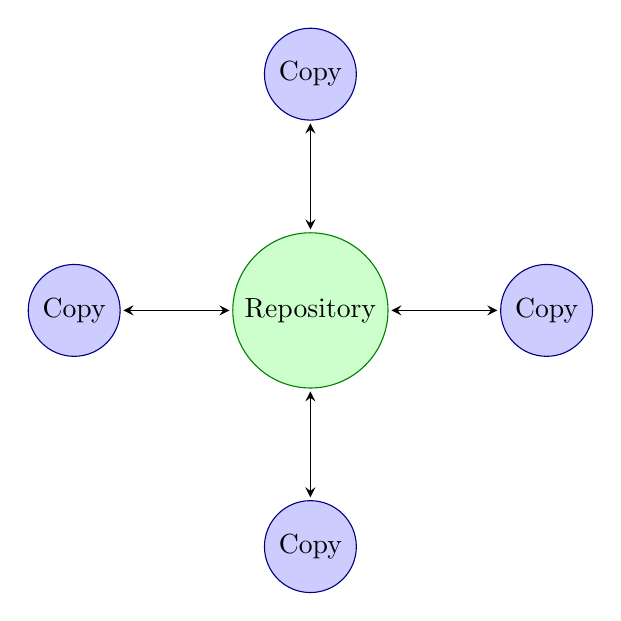
\begin{tikzpicture}
[repo/.style={circle,
		fill=green!20!white,
		draw=green!50!black,
		minimum size=10mm},
workingcopy/.style={circle,
		fill=blue!20!white,
		draw=blue!50!black,
		minimum size=5mm},
link/.style={<->, shorten <=1pt, shorten >=1pt, >=stealth, semithick}]

% central repo
\node at (0, 0) [repo] (mainrepo) { Repository };
% working copies
\node at (3,0)  [workingcopy] (copyright)  { Copy };
\node at (-3,0) [workingcopy] (copyleft)   { Copy };
\node at (0,3)  [workingcopy] (copytop)    { Copy };
\node at (0,-3) [workingcopy] (copybottom) { Copy };
% links between repo and working copies
\draw [link] (mainrepo) -- (copyright);
\draw [link] (mainrepo) -- (copyleft);
\draw [link] (mainrepo) -- (copytop);
\draw [link] (mainrepo) -- (copybottom);
\end{tikzpicture}

        }
    \end{center}
        % -> image/diagram of centralised system
    \begin{itemize}
        \item e.g. Subversion, CVS
    \end{itemize}
    \item Distributed
        % -> image/diagram of distributed system
    \begin{itemize}
        \item e.g. Git, Mercurial
    \end{itemize}
\end{itemize}
\end{frame}

\begin{frame}
\frametitle{Git History}
\begin{itemize}
    \item BitKeeper
    \item License problems
    \item Linux wrote his own system
    \item Open source
\end{itemize}
\end{frame}


%%%%%%%%%%%%%%%%%%%%%%%%%%%%%%%%%%%%%%%%%%%%%%%%%%%%%%%%%%%%%%%%%%%%%%%%%%%%
\section{Installing Git}

\begin{frame}
\frametitle{Installing Git (CLI options)}
\begin{itemize}
    \item Windows
    \item MacOS
    \item Linux/Unix
\end{itemize}
\end{frame}

\begin{frame}
\frametitle{Installing Git (GUI options)}
\begin{itemize}
    \item SourceTree
    \item TortoiseGit
\end{itemize}
\end{frame}

\begin{frame}
\frametitle{Use the Command Line}
\begin{itemize}
    \item With the command line one can get futher and do more; the
        learning curve is steeper, but it's worth it.
    \item Hence, we will focus on the command line interface (CLI) from now
        on.
\end{itemize}
    \blockquote[Hunt and Thomas, \emph{The Pragmatic Programmer}]
    {Gain familiarity with the shell, and you'll find your productivity soaring.}
\end{frame}

\begin{frame}
\frametitle{Text Editors}
\begin{itemize}
    \item Many options:
    \begin{itemize}
        \item Notepad++
        \item Vim, Emacs
        \item Atom
        \item Sublime text
    \end{itemize}
    \item We will be creating and editing text files, hence the need for a
        text editor.
    \item The choice of editor is unimportant; what \emph{is} important is
        that you feel comfortable using yours.
\end{itemize}
\end{frame}

%%%%%%%%%%%%%%%%%%%%%%%%%%%%%%%%%%%%%%%%%%%%%%%%%%%%%%%%%%%%%%%%%%%%%%%%%%%%
\section{Using Git on your own}

\begin{frame}
\frametitle{Using Git on your own}
\begin{itemize}
    \item Why?
    \item Get benefits of version control
    \item Get even more benefits when working with others; we'll discuss
        this in more detail later in the course
    \item Use Git on your local computer
\end{itemize}
\end{frame}

\begin{frame}
\frametitle{Starting a new repository from scratch}
\begin{itemize}
    \item mkdir something
    \item cd something
    \item git init  (also ls -la)
    \item git status
    \item create file
    \item git status (untracked)
    \item git add
    \item git status (staged)
    \item git commit
    \item git status (clean)
    \item git config user.name; git config user.email
    \item master is default branch
    \item (normally don't have to run git status all the time)
\end{itemize}
\end{frame}

\begin{frame}
\frametitle{Starting a new repository (conceptual steps)}
\begin{itemize}
    \item To create a repository, need to \ttt{init}ialise it
        \begin{itemize}
            \item git init
        \end{itemize}
    \item Repository is just a directory, with a .git directory
        \begin{itemize}
            \item ls -la
        \end{itemize}
    \item Things that go into a repository are just files
        \begin{itemize}
            \item touch file
        \end{itemize}
    \item To tell Git to track a file, need to \ttt{add} it
        \begin{itemize}
            \item git add
        \end{itemize}
    \item Tracked files and \emph{changes to tracked files} are put in
        the \emph{staging area}
        \begin{itemize}
            \item git status (see staged)
        \end{itemize}
    \item To record files and \emph{changes to files}, one \ttt{commit}s
        them to the repository
        \begin{itemize}
            \item git commit
        \end{itemize}
\end{itemize}
\end{frame}

\begin{frame}
\frametitle{Exercise: Start a new repository}
\begin{itemize}
    \item Repeat the previous steps on your own computer
    \item Create a directory and change into it
    \item Initialise the repository
    \item Run git status to see the current repository state
    \item Create a file (untracked); see the repository state
    \item Add the file to the repository (track it); see the repository state
    \item Commit the file to the repository; see the repository state
\end{itemize}
\end{frame}

\begin{frame}
\frametitle{Minor Detour: Git Configuration}
\begin{itemize}
    \item Brief intro to git config
    \item Repo-local config
    \item Global config
\end{itemize}
\end{frame}

\begin{frame}
\frametitle{Getting Help}
\begin{itemize}
    \item man pages
    \item git help
    \item books
    \item online references
\end{itemize}
\end{frame}

\begin{frame}
\frametitle{Exercise: git help}
\begin{itemize}
    \item Use \code{git help} on \code{init}, \code{add}, \code{commit} and
        \code{config} commands
    \item Open and browse on \url{https://git-scm.org}
\end{itemize}
\end{frame}

\begin{frame}
\frametitle{Parts of a local Git repository}
\begin{itemize}
    \item Working directory
    \item Staging area
    \item Repository
    \item Very important for understanding operations
    \item need image of wd, staging and repo
\end{itemize}
\end{frame}

\begin{frame}
\frametitle{Snapshots and diffs}
\begin{itemize}
    \item Photograph analogy
    \item Commits build on one another
    \item Working directory: checked out version of local repository
    \item Staging area: what will be committed next
    \item Repository: storage of snapshots
    \item Contrast with other systems, which store diffs between changes
\end{itemize}
\end{frame}

%%%%%%%%%%%%%%%%%%%%%%%%%%%%%%%%%%%%%%%%%%%%%%%%%%%%%%%%%%%%%%%%%%%%%%%%%%%%
\section{Using Git with others}


https://stackoverflow.com/questions/953481/find-and-restore-a-deleted-file-in-a-git-repository

\begin{verbose}
git checkout $(git rev-list -n 1 HEAD -- "$file")^ -- "$file"
\end{verbose}

the file is then shown as a new file in the repo.  One can use `git diff
--cached` to see its contents.

\end{document}

% vim: expandtab shiftwidth=4:
